

\begin{figure}
	\centering
	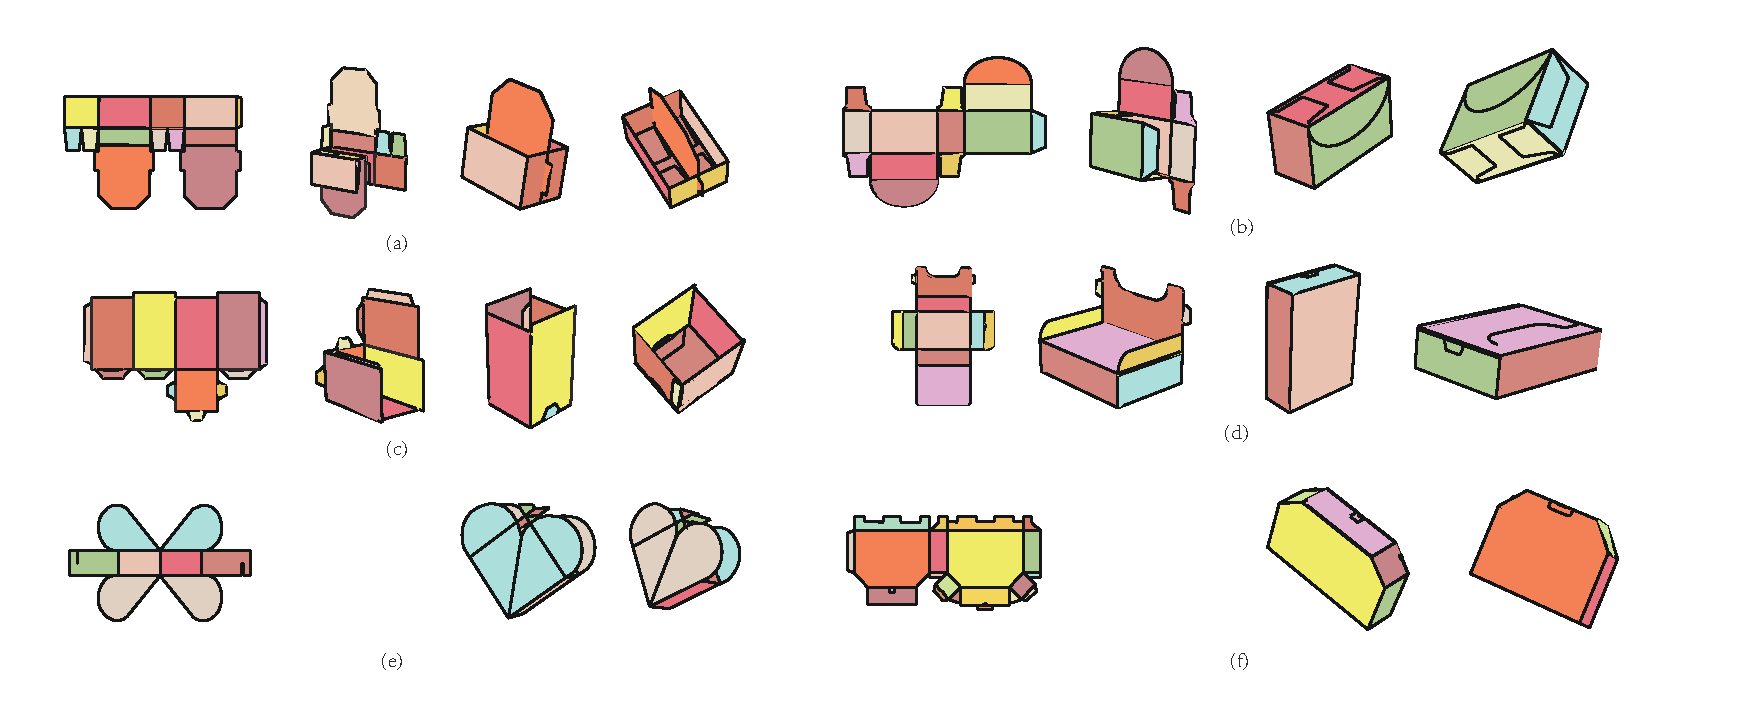
\includegraphics[width=\textwidth]{images/moreAutomatic}
	\caption{More carton examples that can be automatically generated. For each example, four subfigures are shown from left to right: the input 2D layout, an intermediate stage during folding, and the final 3D shape from two views.}  
	\label{fig:automatic-more}
	
\end{figure}

%%%%%%%%%% Results with refinement %%%%%%%%%%

\begin{figure}
	\centering
	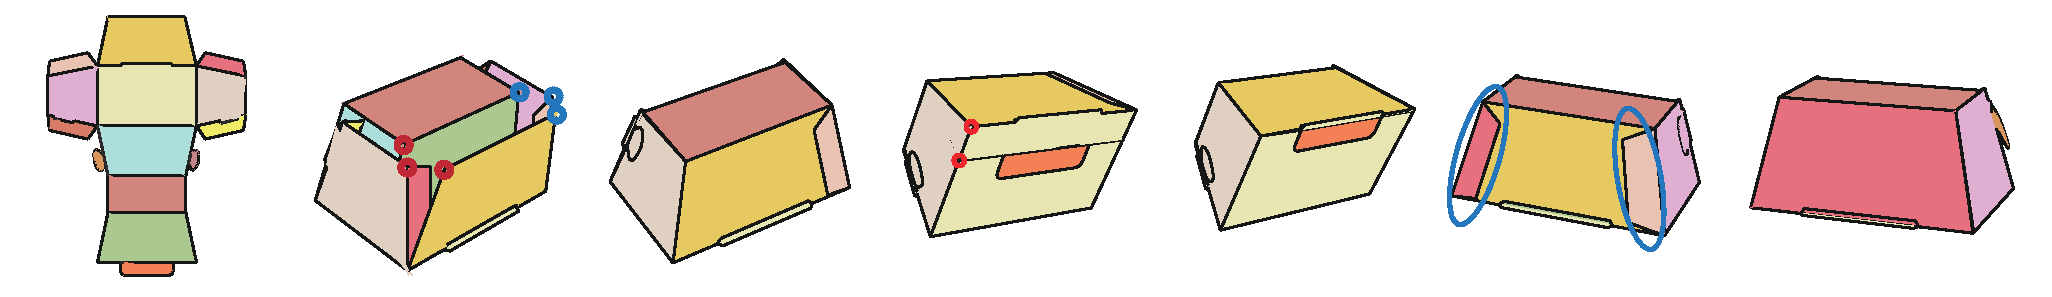
\includegraphics[width=\textwidth]{images/105}
	\caption{The complete process of generating a carton model with user interactions. From left to right: the input structural layout used to generate a flat polymesh, the initial 3D model, two vertex merging confirmations, one panel pasting, and the final 3D model.}
	\label{fig:result}
\end{figure}

\begin{figure}
	\centering
	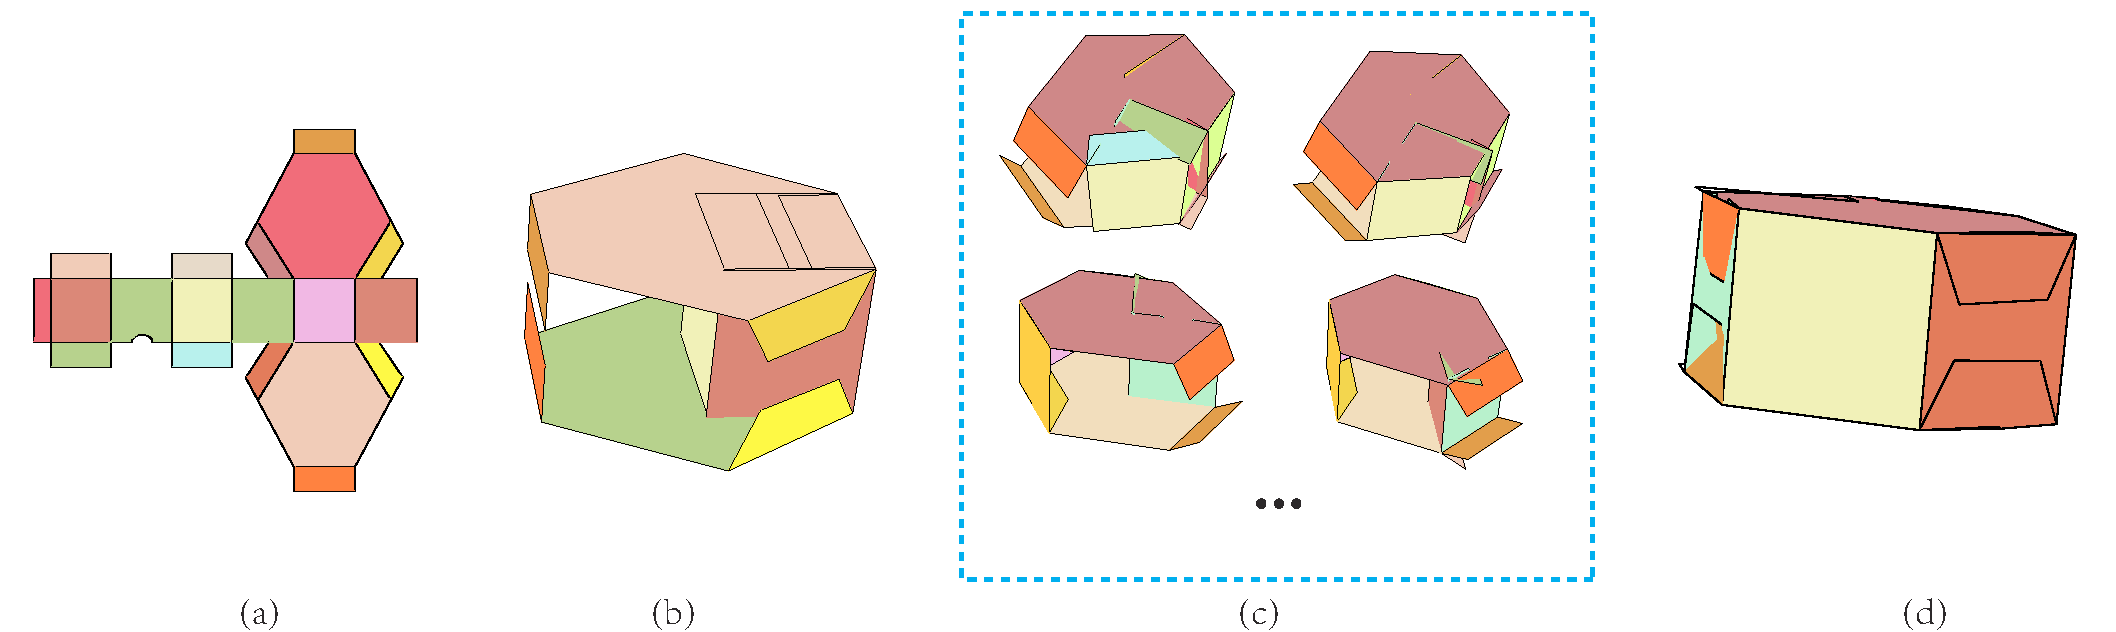
\includegraphics[width=0.9\textwidth]{images/limitation}
	\caption{When given a 2D layout (a), our system generates an initialized result (b). After nine user interactions, including selecting merging vertexes and panel pasting, the final model is obtained as (d). }
	\label{fig:hexagon}
\end{figure}

\begin{figure}[h]
	\centering
	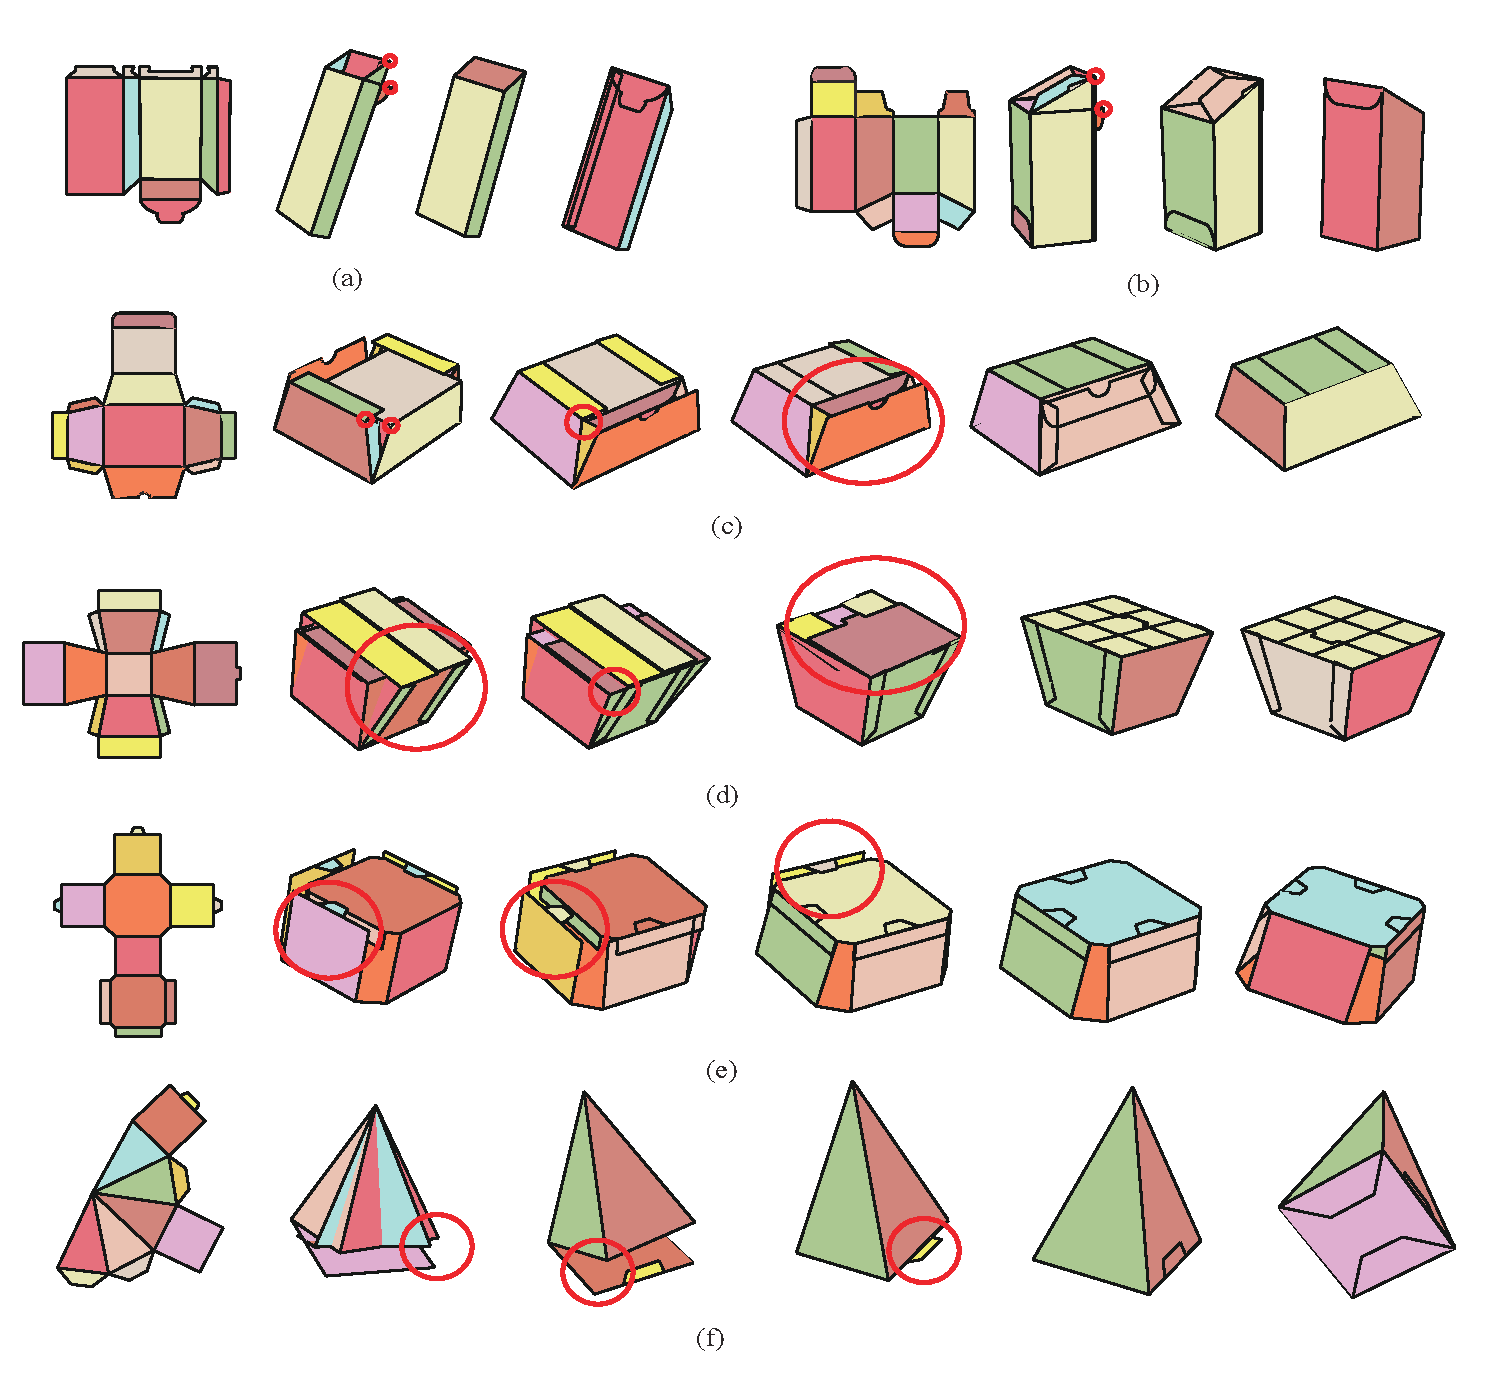
\includegraphics[width=0.9\textwidth]{images/newMore}
	\caption{More complicated results with shape refinement. In each example, the first two images represent the 2D layout and the initial model, and the last two show the final model from different views. The middle images illustrate the intermediate shapes with different shape constraints, which are marked in red circles.}
	\label{fig:result-more}
\end{figure}


\section{Results and Discussion}\label{sec:result}


Based on the two-step approach for folding a carton model, as well as the suggestive user interface, our system is natural and easy to use. 
%
We show a series of results of cartons in various shapes. 
%
A user study was also conducted to examine the effectivenss of our suggestive system.


\subsection{Carton Results}

%%%%%%%%%%% Fully automatic results %%%%%%%%%%%

For most cuboid cartons, their 3D models can be generated by folding each edge by $\pi/2$, as shown in Figure~\ref{fig:initial-automatic} and Figure~\ref{fig:automatic-more}.
%
Nowadays, in the common design process, designers typically spend a great deal of time on manually creating 3D carton models in 3D modeling software. 
Our suggestive interface saves a significant amount of effort, so designers can focus more on designing the appearance of cartons. 


For more complicated cartons, shape refinement is required. 
The entire process of creating a carton model from a 2D layout is illustrated in Figure~\ref{fig:result}.
%
The final model is generated after a total of three clicks: two clicks to confirm vertex merging and one click to confirm panel pasting.
Note that our system automatically detects these possible geometric editing options for users to select; therefore, the user can eliminate the tedious process of selecting edges or vertexes and assigning precise angles or positions to them.
%
A more challenging example is shown in Figure~\ref{fig:hexagon}. 
By initially folding each edge as $\pi/2$, our system first generates a cube inside the carton for the six square faces. 
Occasionally, our system fails to detect the mergeable vertexes with a small threshold $\epsilon$ to merge nearby vertexes; however, the user could manually merge two vertexes. Then, our system automatically detects two symmetric vertexes that also can be merged. 
%
Finally, a hexagonal carton is generated after a limited number of user interactions.
%



More carton models, which were generated using our system with a few user interactions, are shown in Figure~\ref{fig:result-more}.
The statistics of the panel number, edge number, and number of user interactions are listed in Table~\ref{table:statistics}. 
We can see that only a few user interactions are needed for a variety of shapes in order to confirm the system's suggestions.
 

\begin{table}
	\centering
	\caption{Statistics of the number of edges $N_{edge}$, number of panels $N_{panel}$, and the number of user interactions $N_{interaction}$ for the examples shown in this paper.}
	\setlength{\tabcolsep}{1pt}
	\begin{tabular}{c|c|c|c|c|c|c|c|c|c|c|c|c}
		\hline
		Examples & Fig.\ref{fig:automatic-more}(a) & Fig.\ref{fig:automatic-more}(b) &  Fig.\ref{fig:automatic-more}(c) & Fig.\ref{fig:automatic-more}(d) & Fig.\ref{fig:result} & Fig.\ref{fig:hexagon} & Fig.\ref{fig:result-more}(a) & Fig.\ref{fig:result-more}(b)& Fig.\ref{fig:result-more}(c) &  Fig.\ref{fig:result-more}(d) & Fig.\ref{fig:result-more}(e)& Fig.\ref{fig:result-more}(f)\\
		\hline
		$N_{edge}$ & 49 & 62 & 46 & 45 & 54 & 67 & 40 & 43 & 42 & 38 & 48 & 30\\
		$N_{panel}$  & 13 & 13 & 11 & 13 & 14 & 19 & 11 & 13 & 13 & 13 & 12 & 11\\
		$N_{interaction}$  & 0 & 0 & 0 & 0 & 3 & 9 & 1 & 4 & 1 & 3 & 3 & 3\\ 
		\hline
		\end{tabular}
		\label{table:statistics}
\end{table}


%%%%%%% User Study %%%%%%%%%%%%%%%%%%%%%%%%%%%%%
 
\subsection{User Study}
\label{sec:userstudy}
 
 
 \begin{figure}  
 	\centering
 	\subfigure[System Preference]{
 		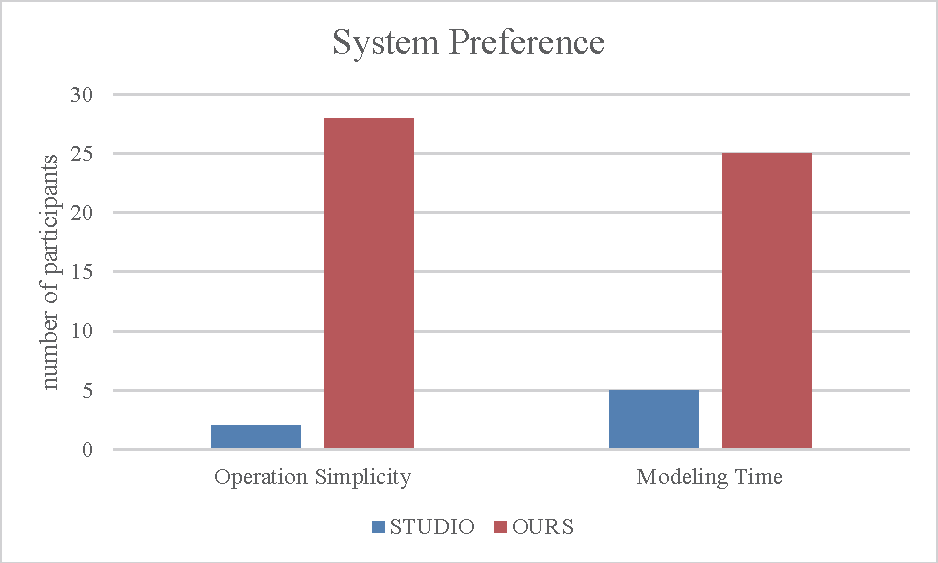
\includegraphics[width=0.25\columnwidth,height=0.11\textheight]{images/preference}
 		\label{fig:preference}
 	}
 	\vspace{2ex}
 	\subfigure[Layout Refinment]{
 		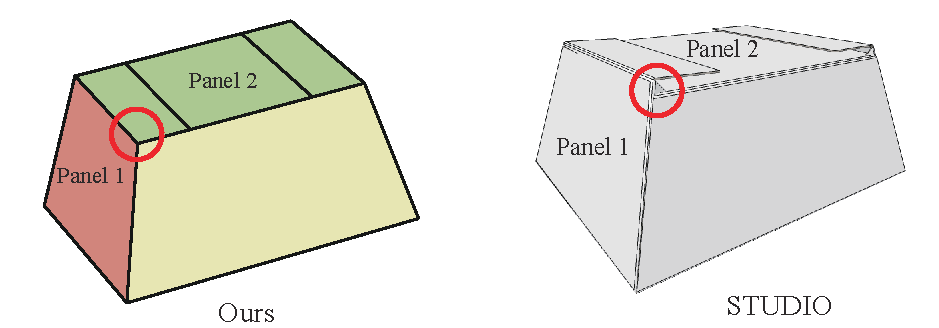
\includegraphics[width=0.35\columnwidth,height=0.08\textheight]{images/comparison}
 		\label{fig:correction}
 	}
 	\vspace{2ex}
 	\subfigure[Fabrication Time]{
 		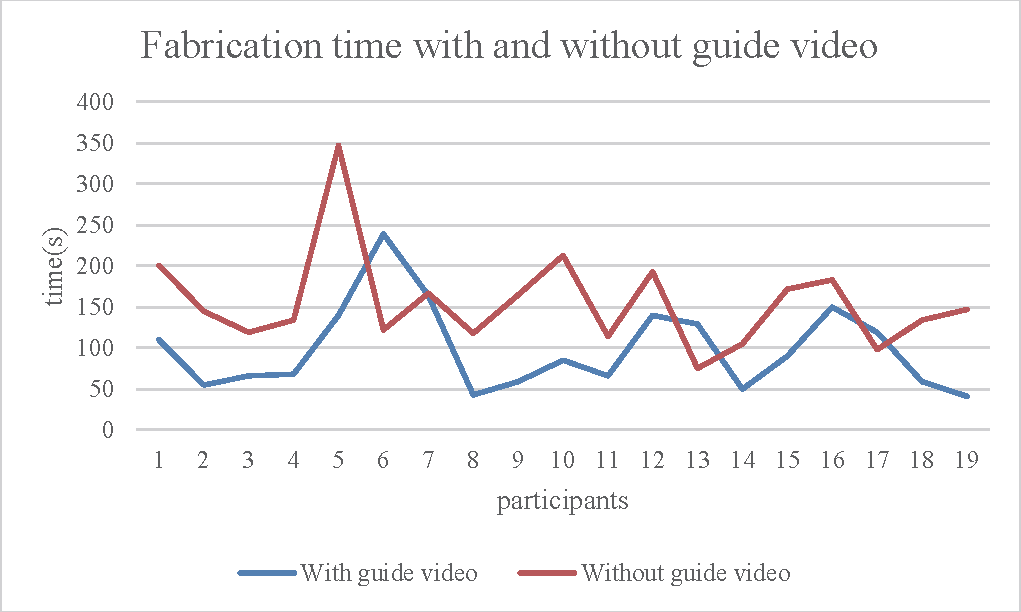
\includegraphics[width=0.25\columnwidth,height=0.11\textheight]{images/fabrication}
 		\label{fig:time}
 	}
 	\caption{(a) Compared with STUDIO, more participants prefer our system with regard to both the operation simplicity and modeling time. (b) Our system is able to automatically refine the inaccurate 2D layout, while STUDIO only generates the folded shape based on user assigned angles. (c) Comparison of fabrication times with/without video. It took much longer for common users to fabricate a carton from a 2D layout without our guide.}
 	\label{fig:userstudy}
 \end{figure}
 
 
 
We conducted a user study to examine the productivity of our system for constructing digital 3D mockups from 2D layouts and to analyze the effectiveness of our system in guiding non-expert users to fabricate physical mockups from 2D layouts. 
%
There are two experiments in our user study.
% 
In the first experiment, participants were given a brief introduction, and then they were asked to construct a digital 3D model from the same 2D layout using our system and the commercial software, STUDIO, respectively.
For each participant, 10 examples were randomly selected from the 34 2D design layouts and presented to the participant for folding using our system and STUDIO.
A \emph{two-alternative forced choices} design was used, so the participant was asked to choose which of the two systems they would prefer to use after considering operation simplicity and modeling efficiency. 
%
Furthermore, participants were asked to rate the necessity of layout optimization in our system by using a scale from one to five, with five indicating that it is very necessary.

%
In the second experiment, participants were separated equally into two groups. One group was asked to fold a sheet of paper into a physical carton. The 2D layout was printed onto this piece of paper, and the user was guided by a video showing the folding sequence according to our system. Another group was asked to make a carton without the guide video. 
Each participant was assigned with the same 2D layout (Figure~\ref{fig:automatic-more}(a)), because it is not easy to imagine the final mockup from the 2D layout at first sight.
%
The fabrication times were recorded for the two groups.
%

Based on the two experiments, our goal was to test the following hypotheses:

\begin{itemize}
	\item \textbf{Hypo1:} Our system takes less time and effort to construct a digital 3D mockup than the traditional software.
	\item \textbf{Hypo2:} Our system provides novel and practical functions for generating diverse layouts.
	\item \textbf{Hypo3:} Our system is effective for guiding non-expert users to fabricate complex cartons from 2D layouts.
\end{itemize}




We consider our three hypotheses in turn. 
With respect to \textbf{Hypo1}, we collect the answers to the former two questions from 30 participants, all over eighteen years of age. Both male and female participants were included, and none had any prior experience with designing or folding cartons in computer software. 
%
The results are shown in Figure~\ref{fig:preference}. 
The chart shows that $93\%$ of participants prefer our system with regard to the operation simplicity, and $83\%$ of participants prefer our system with regard to the modeling time.
%
We also performed a paired-samples $t$-test at the level $\alpha = 0.05$ to compare the preference significance.
%
This test shows that our system is significantly preferred by participants.
%
Most participants voted for our system because it takes much less time to make a 3D model using our system. 
Take Figure~\ref{fig:result-more}(e) for example, participants usually spent much time adjusting the folding angles of the creases, while only three clicks are required in our system.
%
On the other hand, one comment from the participants who preferred STUDIO stated that the operation in STUDIO only required them to select and assign angles, while our system required them to learn more operations to construct the digital 3D model. 
%

With respect to \textbf{Hypo2}, 24 participants gave the highest score to our layout optimization function. 
%
In addition to exploring the diversity of 2D layouts, our system can also adjust the imprecise panels on the 2D layout to reach an ideal model. Figure~\ref{fig:correction} shows the final models constructed by our system and STUDIO, respectively. As we can see, Panel 1 is higher than Panel 2 in the digital model constructed by STUDIO, because the 2D layout is not as precise as the designer would like. 
%
In comparison, our system is able to correct these design errors by merging the 3D vertexes in different panels, which are circled in red. This step optimizes the corresponding 2D layout.
 
 
Considering \textbf{Hypo3}, 38 participants (19 in each group) were asked to transform the 2D layout shown in Figure~\ref{fig:automatic-more}(a) into a physical carton. 
The comparison of the fabrication times with and without our guide video is shown in Figure~\ref{fig:time}. 
As we can see, most participants who did not watch the guide video spent more time, averaging 155 seconds, to fold a carton than the other group, averaging 99 seconds.
% 
%
We also performed an independent-samples $t$-test at the level $\alpha = 0.05$ to compare the fabrication times. The results show that the guide video is a highly effective tool for non-expert users in fabricating complex cartons. 





\paragraph{Limitations.}

\begin{figure} 
	\centering
	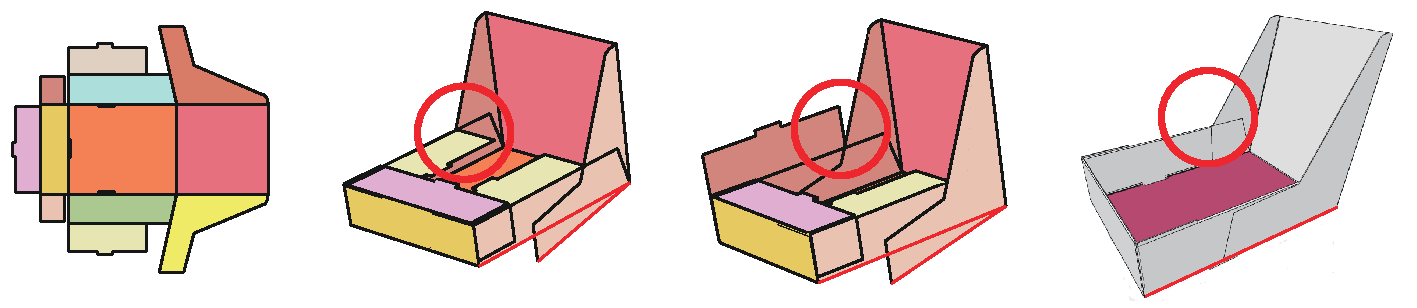
\includegraphics[width=0.8\textwidth]{images/moreLimitation}
	\caption{Limitations in our current system. From left to right: a 2D layout, the initial model after folding each edge by $\pi/2$, the optimized model after pasting the three panels circled in red, and the desired carton model constructed from the 2D layout. }
	\label{fig:failure}
\end{figure}

%%%%%%%%%% Limitations and discussions %%%%%%%%%%%%%%%%%%%%%%%%%%%%%%%%%

Our suggestive shape optimization is very useful in a wide range of cases. Nevertheless, there are still some failure cases that our system can not deal with. Figure~\ref{fig:failure} shows a case that is challenging for our current system. The panels circled in red should be pasted together to produce a strong enforced panel.
However, our system only ensures the coplanarity of the selected three panels, and as a result, the yellow panel is expanded in the opposite direction. 
%
Moreover, the pink back panel is orthogonal to the bottom panel after initialization, and the two red edges are not aligned.   
This can be solved by adding more editing tools, such as aligning edges, or assigning a folding angle for a specific edge, such as STUDIO.

